\documentclass[a4paper,fleqn,12pt]{article}
\usepackage[utf8]{inputenc}
\usepackage{tikz}
\usepackage{amsmath}
\usepackage{cancel}
\usepackage[estonian]{babel}

%yl2
\usepackage{indentfirst}

%yl4
\usepackage{icomma}

%yl5:
\usepackage{xstring}
\usepackage{ifthen}

%yl6
\usepackage{amsthm}
\theoremstyle{definition}
\newtheorem*{solution}{\indent\textmd{\emph{Lahendus}}}
\newtheorem*{answer}{\indent\textmd{\emph{Vastus}}}

%yl7
\usepackage{pst-eucl}
\usetikzlibrary{arrows,calc}

%yl8
\newtheorem{definition}{Definitsioon}[section]
\usetikzlibrary{fit,arrows,positioning}
\renewcommand{\figurename}{Joonis}
\renewcommand{\tablename}{Tabel}
\renewcommand\refname{}
\usepackage{amssymb}

%ylt
\usepackage{soulutf8}
\usepackage{gensymb}

\begin{document}

\begin{titlepage}
	\begin{center}
	
		\uppercase{Tartu Ülikool}\\[2mm]
		\uppercase{Matemaatika-Informaatikateaduskond}\\[2mm]

		\vspace{6cm}

		{\Huge Rakendustarkvara: \TeX}\\[2mm]
		{\large praktikumitöö}

		\vspace{6cm}

		\begin{flushright}
			\Large
			Rauno Viskus\\[2mm]
			MatStat, 3.
		\end{flushright}

		\vfill

		{\large Tartu 2014}
	\end{center}
\end{titlepage}
\section{Ülesanne 2.}

\subsection*{}

Tõestame teoreemi kahe teguri korrutise kohta, millest järeldub teoreemi kehtivus.
Olgu $\log_a b_1 = x_1$ ja $\log_a b_2 = x_2$, siis $b_1 = a^{x_1}$ ja $b_2 = a^{x_2}$. Leiame arvude $b_1$ ja $b_2$ korrutise: $b_1 b_2 = a^{x_1} a^{x_2}$ ehk $b_1 b_2 = a^{x_1 + x_2}$. Logaritmi definitsiooni järgi saame viimasest võrdusest, et $\log_a(b_1 b_2) = x_1 + x_2$. Asendades $x_1$ ja $x_2$ vastavate logaritmidega, saame:
\begin{displaymath}
	\log_a(b_1 b_2) = \log_a b_1 + \log_a b_2
\end{displaymath}

\subsection*{}

Kahe nurga vahe ja summa tangensi valemite tuletamiseks kasutame ühe ja sama nurga trigonomeetriliste funktsioonide vahelisi põhiseoseid ja eespool saadud valemeid:
\begin{displaymath}
	\tan(\alpha	- \beta)
		= \frac{\sin(\alpha	- \beta)}{\cos(\alpha	- \beta)}
		= \frac{\sin\alpha\cos\beta - \cos\beta\sin\alpha}
					 {\cos\alpha\cos\beta + \sin\alpha\sin\beta}
\end{displaymath}

\subsection*{}

Lahenda võrrandisüsteem
\begin{displaymath}
  \begin{array}{*{7}{r}}
    x  & + & 2y & + &  z = &  5, \\
    4x & - &  y & + & 2z = & -3, \\
    2x & + & 3y & + & 4z = &  3. \\
  \end{array}
\end{displaymath}
Lahendus.
\begin{displaymath}
	D = 
	\begin{array}{|*{3}{r}|}
	1 & 2 & 1 \\
	4 & -1 & 2 \\
	2 & 3 & 4 \\
	\end{array}
	= -4 +12 +8 +2 -32 -6 = -20.
\end{displaymath}
\section{Ülesanne 3.}


\subsection*{}

\begin{center}
  $\begin{array}{ | r | *{8}{c} | }
    \hline
    \multicolumn{1}{|c|}{\text{Esimesed}} & \multicolumn{8}{|c|}{\text{Viimased kolm tähte}} \\
    \text{kaks tähte} & aaa & aab & aba & abb & baa & bba & bab & bbb \\ \hline
    aa & 2 & 2 & 2 & 2 & 5 & 7 & 5 & 7 \\
    ab & 3 & 4 & 4 & 4 & 1 & 2 & 0 & 2 \\
    ba & 0 & 1 & 0 & 0 & 3 & 5 & 3 & 5 \\
    bb & 5 & 6 & 6 & 6 & 2 & 2 & 2 & 2 \\
    \hline
  \end{array}$
\end{center}

\subsection*{}

\begin{center}
  \begin{tabular}{ r @{ $=$ } l }
					   $f(x+\Delta x)$ & $3(x + \Delta x)^2 + 2$ \\
					            $f(x)$ & $3x^2  + 2$ \\
    \hline
    $f(x+\Delta x)$ - $f(x)$ & $3(x + \Delta x)^2 + 2 - (3x^2  + 2)$.
  \end{tabular}
\end{center}
\newcommand{\cOut}[2]{
\stackrel{\textstyle #2}{\cancel{#1}}
}

\newcommand{\cOutB}[2]{
\underset{\textstyle #2}{\cancel{#1}}
}

\section{Ülesanne 4.}

\subsection*{}

\begin{displaymath}
  A = \lim_{\Delta x \to 0} \sum_{x=0}^{h} 9810 \pi r^2 x \: \Delta x \: \mathrm{J}.
\end{displaymath}

\subsection*{}

\begin{displaymath}
  a^m : a^n =
  \frac{a^m}{a^n} =
  \frac{\overbrace{aa \dots a}^\text{$n$ tegurit} \cdot \overbrace{aa \dots a}^\text{$m-n$ tegurit}}
  {\underbrace{aa \dots a}_\text{$n$ tegurit}} =
  a^{m-n}.
\end{displaymath}

\subsection*{}

\begin{displaymath}
  \begin{split}
    & S = \int\limits_0^9 3\sqrt{x} \mathrm{d}x - \int\limits_0^9 x \mathrm{d}x =
    3 \int\limits_0^9 x^{\frac{1}{2}} \mathrm{d}x - \int\limits_0^9 x \mathrm{d}x =
    3\left[\frac{x^{\frac{3}{2}}}{\frac{3}{2}}\right]_0^9 - \left[\frac{x^2}{2}\right]_0^9 = \\
    & 2[x \sqrt{x}]_0^9 - \frac{1}{2} [x^2]_0^9 =
    2 \cdot 27 - \frac{1}{2} \cdot 81 = 54 - 40,5 = 13,5 \: \text{ruutühikut}.
  \end{split}
\end{displaymath}

\subsection*{}
  Näiteks $15^4 : 5^4 = (15 : 5)^4 = 3^4 = 81$.
\par
Viimase tehte õigsus on eriti hästi näha, kui kirjutada jagamine murruna ja siis murdu taandada.
\begin{displaymath}
  \frac{15^4}{5^4} = \frac{\cOut{15}{3} \cdot \cOut{15}{3} \cdot \cOut{15}{3} \cdot \cOut{15}{3}}{\cOutB{5}{1} \cdot \cOutB{5}{1} \cdot \cOutB{5}{1} \cdot \cOutB{5}{1}} = 3^4 = 81.
\end{displaymath}
\newcommand{\tooLong}[2]{%
\StrLen{#1}[\theLength]%
\ifthenelse{ \theLength > #2 }{%
  \StrLeft{#1}{#2} \dots%
}{%
  #1%
}%
}

\newcommand{\weekDays}{
\foreach \d/\a in {esmaspäev/E, teisipäev/T, kolmapäev/K, neljapäev/N, reede/R, laupäev/L, pühapäev/P}{
  \noindent\d(\a)\\
}
}

\section{Ülesanne 5.}

\subsection{Parameetriga makro}

Eelmise ülesande lahendamiseks defineeritud taandamise makro:
\begin{displaymath}
  \cOut{90}{123} \quad \text{ja} \quad \cOutB{321}{123}
\end{displaymath}

\subsection{Hargnemisega makro}

Käsk, mis lühendab teksti maksimmalselt etteantud pikkuseks. Kui teksti lühendatakse märgitakse see ära kolme punktiga:

Parameetritega '123456' ja 5: \tooLong{123456}{5}

Parameetritega '1234' ja 5: \tooLong{1234}{5}

\subsection{Tsükliga makro}

Makro nädalapäevade välja trükkimiseks. Ülikasulik kui on vaja korduvalt igal pool nädalapäevi välja trükkida(produktiivsusgarantii):

\weekDays
\section{Ülesanne 6.}

\begin{solution}
Koostame võrrandisüsteemi ja lahendame selle liitmisvõttega (V ptk., art. 7):
\begin{displaymath}
\begin{array}{rr}
	\left\{
	\begin{array}{*{3}{r@{}}}
	 x + 2y&-&2=0  \\
	2x + y&-&13=0
	\end{array}
	\right.

	\quad

	\left|
		\begin{array}{c}
		\cdot2\\
		\cdot(-1) 
		\end{array}
	\right|&
	+
	\begin{array}{r@{\,}l}
		2x+4y-4 &=0\\
		-2x-y+13&=0
	\end{array} 
	\\
	& 3y+9=0;\\
	& y=-3.
\end{array}
\end{displaymath}

\end{solution}

Nüüd asendame esimeses võrrandis $y$ arvuga $-3$ ja leiame $x$ väärtuse:
\begin{displaymath}
x+2\cdot(-3)-2=0 \Rightarrow x=8.
\end{displaymath}

\begin{answer}
Sirgete lõikepunkt on $(8; -3)$.
\end{answer}
\section{Ülesanne 7.}

\subsection*{}

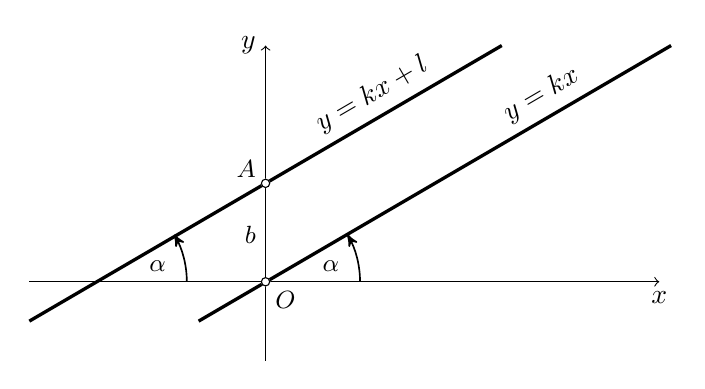
\begin{tikzpicture}

	%X axis
	\draw [->] (-3,0) -- (5,0) node[below] {$x$};
	%Y axis
	\draw [->] (0,-1) -- (0,3) node[left] {$y$};

	\draw [very thick] (-3,-0.5) -- (3,3) node [sloped,above,near end] {$y=kx+l$};
	\draw[->,>=stealth',semithick] (0cm:-1cm) arc (0:30:1.2cm);
	\draw (-1.6cm, 0cm) node[above right] {\small $\alpha$};

	\draw [very thick] (-0.85,-0.5) -- (5.15,3) node [sloped,above,near end] {$y=kx$};
	\draw[->,>=stealth',semithick] (0cm:1.2cm) arc (0:30:1.2cm);

	\draw (.6cm, 0cm) node[above right] {\small $\alpha$};


	\draw (0cm, 1.2cm) node[above left] {\small $A$};
	\draw[fill, white] (0,1.25) circle [radius=1.5pt];
  \draw (0,1.25) [thin] circle (1.5pt);

	\draw (0cm, 0cm) node[below right] {\small $O$};
	\draw[fill, white] (0,0) circle [radius=1.5pt];
  \draw (0,0) [thin] circle (1.5pt);

	\draw (0cm, 0.6cm) node[left] {\small $b$};

\end{tikzpicture}


\subsection*{}

\begin{tikzpicture}
	%X axis
	\draw [->] (-2,0) -- (6,0) node[below] {$x$};
	%Y axis
	\draw [->] (0,-1) -- (0,4) node[left] {$y$};

	\draw (-1.5,2) -- (5.5,2) node [sloped,above,very near end] {$y=b$};

	\foreach \xCoordinate in {-0.5, 1, 2.5}{
		\draw [<->,>=latex] (\xCoordinate,0) -- (\xCoordinate,2cm) node [midway,left] {$b$};
	}

	\foreach \letter/\position in {B/1, C/2.5}{
		\draw (\position, 2cm) node[above] {\small $\letter$};
		\draw[fill, white] (\position, 2cm) circle [radius=1pt];
	  \draw (\position, 2cm) [thin] circle (1pt);		
	}

	\draw (0cm, 0cm) node[below right] {\small $O$};
	\draw[fill, white] (0,0) circle [radius=1pt];
  \draw (0,0) [thin] circle (1pt);


	\draw (0cm,2cm) node[above left] {\small $A$};
	\draw[fill, white] (0cm,2cm) circle [radius=1pt];
  \draw (0cm,2cm) [thin] circle (1pt);

\end{tikzpicture}


\subsection*{}


\begin{tikzpicture}

  \begin{scope}
    \clip (0,0) circle (3cm);
    \fill[black] (3cm,3cm) rectangle (-3cm, -3cm);
    %fill[color] (right,top) rectangle (left,bottom);
  \end{scope}

  \begin{scope}
    \clip (-1,0) circle (2cm);
    \fill[white] (3cm,3cm) rectangle (-3cm, -0.01cm);
  \end{scope}

  \begin{scope}
    \clip (1,0) circle (2cm);
    \fill[white] (3cm,0.01cm) rectangle (-1cm, -2cm);
  \end{scope}

  \fill[black] (2,0.05) circle (1cm);
  \fill[black] (-2,-0.05) circle (1cm);

  \draw (0,0) [ultra thick] circle (3cm);

\end{tikzpicture}
\section{Ülesanne 8.}

\subsection{Teoreem}

\begin{definition}[Varjatud Markovi ahel]%~\citep{lember10}
	Protsessi $X = \{Y_t\}_{t\geqslant1}$ nimetatakse varjatud Markovi ahelaks kui kehtib:

	\begin{enumerate}
		\item $\{Y_t\}_{t\geqslant1}$ korral, juhuslikud suurused $\{X_t\}_{t\geqslant1}$ on omavahel sõltumatud;
		\item iga $t = 1,2,\dots$, korral on $X_t$ sõltuv juhuslikust protsessist $\{Y_t\}_{t\geqslant1}$ (ja ajast $t$) ainult läbi $Y_t$.
	\end{enumerate}

	Juhuslike protsesside paarile $(X, Y)$ viidatakse ka kui \textit{varjatud Markovi mudelile}.
\end{definition}

\subsection{Tabel}

\begin{table}[h]
	\centering
	\begin{tabular}{ r | *{4}{c} }	
						& SV 	& sport & sots. & nutt\\
		\hline
			 kurb & 0,3 & 0,15	 & 0,05 & 0,5 \\
		õnnelik & 0,2	& 0,2   & 0,5	& 0,1 \\
	\end{tabular}

	\caption{Emissioonitõenäosused.}
	\label{fig:HMM.ex.emission}
\end{table}

\subsection{Joonis}

Varjatud Markovi ahela mõistet võib kujutada ka järgneva skeemiga:

\begin{figure}[h]
	\centering
	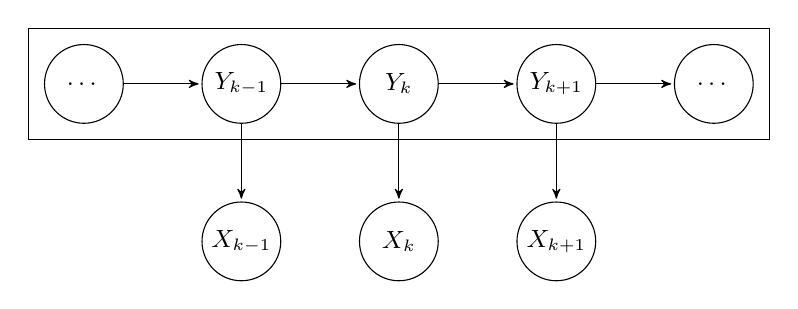
\begin{tikzpicture}[
		->,
		>=stealth',
		shorten >=1pt,
		auto,
		node distance=2cm,
		main node/.style={inner sep=0cm,circle,minimum width=1cm,fill=white,draw,font=\small}]

	\node[main node] (y1) {\dots};
	
	\node[main node] (y2) [right of=y1] {$Y_{k-1}$};
	\node[main node] (x2) [below of=y2] {$X_{k-1}$};
	
	\node[main node] (y3) [right of=y2] {$Y_{k}$};
	\node[main node] (x3) [below of=y3] {$X_{k}$};
	
	\node[main node] (y4) [right of=y3] {$Y_{k+1}$};
	\node[main node] (x4) [below of=y4] {$X_{k+1}$};
	
	\node[main node] (y5) [right of=y4] {\dots};
	
	\node[rectangle, inner sep=2mm,draw=black!100, fit=(y1) (y2) (y3) (y4) (y5)] {};

	\path
		(y1) edge node {} (y2)
		(y2) edge node {} (y3)
		(y3) edge node {} (y4)
		(y4) edge node {} (y5)
		
		(y2) edge node {} (x2)
		(y3) edge node {} (x3)
		(y4) edge node {} (x4)
	;
\end{tikzpicture}

	\caption{Varajtud Markovi ahela kuju.}
	\label{fig:HMM}
\end{figure}

Joonisel~\ref{fig:HMM} ristküliku sees olev osa on meile üldjuhul vaadeldamatu ja sealt tuleb varjatud Markovi ahelatele ka nimi.

\subsection{Kirjanduse loetelu}

\begin{thebibliography}{99}

\bibitem{Knuth84} D. E. Knuth. The {\TeX}book.
Addison-Wesley, 1984.

\bibitem{lamport94} Leslie Lamport,
	\emph{\LaTeX: A Document Preparation System}.
	Addison Wesley, Massachusetts,
	2nd Edition,
	1994.

\bibitem{thebestbookintheworld} Eno Raud,
  Sipsik.
  Eesti raamat,
  1962.
\end{thebibliography}

\section{Ülesanne 9.}

Idee mida \TeX{} kannab on hea. Mulle meeldib, et saan tavalises tekstivormis oma soovi kirjeldada ning oman seega paremat kontolli tulemuse üle ning olen sarnaseid vahendeid kasutanud ka varajasemalt nii palju kui võimalik(Mark\-downi formaadis).

Samuti kiidan filosoofiat vormistuse korra ja reeglite aspektist, mida \TeX{} justkui "peale surub". Kui tõstame esile sisu ning laseme vormil olla täiesti eraldatud võidavad kõik - nii loov kui tarbiv pool. Sinna suunas liigub ka kogu ülejäänud loov kammuun. Veebiarendus on hea näide.

Teisalt aga leian, et see tööriist on vanamoodne ning ehk aegunudki, kuigi hea alternatiiv puudub. Makrod on kasutamatud ning loetamatu süntaksiga, paketimajanduse haldamine ja konfigureerimine kaootiline, tihti viletsa dokumentatsiooniga ning "automaagilisel" viisil töötav. Süsteemi ülesehitus on kohmakas ja platvorm ise suur ning takistab suuresti normaalset arengut (nagu ma aru saan pakendatakse kõik lisapaketid/moodulid, liveTexiga näiteks, esmasel installil kaasa).

\TeX ile kuluks ära paketihaldur(nagu npm, mis tooks kaasa pakettide versioonihalduse ning sõltuvus hierarhia) ning viis integreerida tex failidega mingit programmeerimiskeelt("inline coding": javascript. ruby, kasvõi php). Viimast ideed kujutan hästi ette ka praegu rakendatavat - tex fail tuleb eelnevalt lihtsalt ühe korra veel läbi käia vastava keele parseri või interpretaatoriga.

Sai mõni lause rohkem kui paar.
\section{Ülesanne 10.}


\indent\so{Näide 4}. Nurga radiaanmõõt on 2,495. Arvutada selle nurga kraadimõõt.
\begin{solution}
Valemi (2) järgi saame:
\begin{displaymath}
\alpha = \frac{2,495 \cdot 180 \degree}{\pi} = \frac{2,495 \cdot 180 \degree}{2,14} = 143 \degree.
\end{displaymath}
Kasutades radiaanmõõdu definitsiooni, on kerge tuletada valem kaare pikkuse leidmiseks: et $a=\frac{l}{R}$, siis $l=aR$, s.t. kaare pkkus võrdub kaare radiaanmõõdu ja raadiuse korrutisega.
\end{solution}

\subsection{Trigonomeetriliste funktsioonide üldistatud definitsioonid}

Käesoleva peatüki artiklis 1 defineerisime teravnurga trigonomeetrilised funktsioonid. Need definitsioonid aga pole rakendatavad nürinurga ja negatiivse nurga korral, sest nad ei anna vastust küsimusele: mida nimetatakse nürinurga või negatiivse nurga trigonomeetrilisteks funktsioonideks. On ilmne, et kuitahes suurte ja mistahes märgiga võetud nurkade trigonomeetriliste funktsioonide käsitlemisel tuleb üldistada trigonomeetriliste funktsioonide mõistet ja defineerida trigonomeetrilisi funktsioonie selliselt, et need sisaldaksid endas ka teravnurga trigonomeetriliste funktsioonide definitsioone kui erijuhte.

Võtame koordinaattasandi alguspunkti ümber vabalt pöörleva kohavektori $\overrightarrow{OA}$, mille lõpp-punkti koordinaadid on $x$ ja $y$ ning moodul $r$ (joon. \ref{fig:theGreatCircle}). Pöörlemisel moodustab kohavektori lõpp-punkt ringjoone, raadiusega $r$. Nimetame seda ringjoont


\begin{figure}[h]
	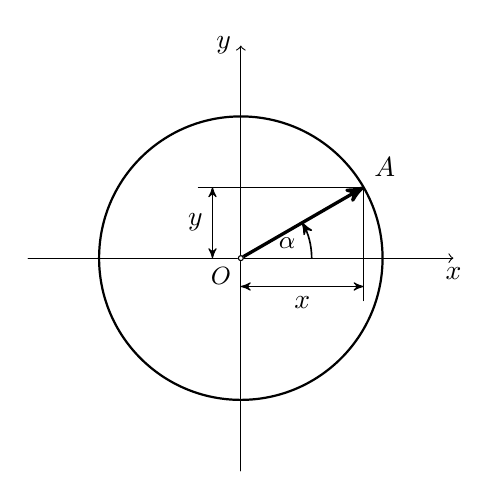
\begin{tikzpicture}[scale=1.8,cap=round]
		\tikzstyle{important line}=[very thick]
		\def\costhirty{0.8660256}

		%axes
		\draw [->] (-1.5,0) -- (1.5,0) node[below] {$x$};
		\draw [->] (0,-1.5) -- (0,1.5) node[left] {$y$};
		%circle
		\draw[thick] (0cm,0cm) circle(1cm);
		%pointA
		\draw[->,>=stealth',very thick] (0cm,0cm) -- (30:1cm) node [above right] {$A$};
		%angle
		\draw[->,>=stealth',semithick] (0cm:0.5cm) arc (0:30:0.5cm);
		\draw (.2cm, 0cm) node[above right] {\small $\alpha$};

		%lines
		\draw (\costhirty,0.5) -- (-0.3,0.5);
		\draw (\costhirty,0.5) -- (\costhirty,-0.3);

		%lengths
		\draw [<->,>=stealth'] (-0.2,0) -- (-0.2,0.5) node [midway,left] {$y$};
		\draw [<->,>=stealth'] (0,-0.2) -- (\costhirty,-0.2) node [midway,below] {$x$};

		%origin
		\draw (0cm, 0cm) node[below left] {\small $O$};
		\draw[fill, white] (0,0) circle [radius=.5pt];
		\draw (0,0) [thin] circle (.5pt);
	\end{tikzpicture}
	\caption{\hspace{375pt}}
	\label{fig:theGreatCircle}
\end{figure}

\end{document}
